\documentclass[12pt,a4paper]{report}
\usepackage[utf8]{inputenc}
\usepackage{amsfonts}
\usepackage{setspace}
\usepackage{graphicx}
\usepackage{array}
\usepackage{fancyhdr}
\linespread{1.5}
\usepackage{geometry}
\parindent 0px
\geometry{
a4paper,
total={210mm,297mm},
left=1.25in,
right=0.75in,
top=0.75in,
bottom=0.75in,
}

\begin{document}
\pagestyle{empty}
\begin{center}
{\large \textbf{VISVESVARAYA TECHNOLOGICAL UNIVERSITY}}
\par
\vspace{3pt}
{\large \textbf{``JNANA SANGAMA'', BELAGAVI - 590 018}}
\begin{figure}[hbtp]
\centering

\includegraphics[width=0.80in,height=0.75in]{../fig/vtu}
\end{figure}
\\
\textbf{A MINI PROJECT REPORT}
\par
\textbf{on}
\par 
\vspace{3pt}
{\Large \textbf{`` ARMS AND AMMUNITION SYSTEM  ''}}
\par
\vspace{8pt}
\textit{\textbf{Submitted by}}
\par
\vspace{6pt}
\textbf{\large Krishna G Kamath}\hspace{0.9in}\textbf{\large \hspace{0.25in}4SF18IS044}\\
\textbf{\large Mayur Pai B H}\hspace{1.5in}\textbf{\large 4SF18IS053}\\
\par
\vspace{3pt}
\textit{\textbf{In partial fulfillment of the requirements for the V semester }}
\par
\vspace{0.5pt}
\Large \textbf{DBMS LABORATORY WITH MINI PROJECT}
\par
\vspace{0.5pt}
\normalsize \centering \textbf{of}
\par
\vspace{0.5pt}
\large \textbf{BACHELOR OF ENGINEERING }
\par
\vspace{0.5pt}
\textbf{in}
\par
\vspace{0.5pt}
\large \textbf{INFORMATION SCIENCE \& ENGINEERING}
\par
\vspace{2pt}
\textit{\textbf{Under the Guidance of}}
\par
\vspace{6pt}
\textbf{\large Mr. Rithesh Pakkala P.}\\
\normalsize\textbf{ Assistant Professor}\\
\normalsize\textbf{Department of ISE}\\
\par
\vspace{0.5pt}
\normalsize \centering \textbf{at}\\
\begin{figure}[hbtp]
\centering

\includegraphics[width=1.0in,height=0.85in]{../fig/sahyadri}
\end{figure}
{\LARGE \textbf{SAHYADRI}}
\par
\vspace{6pt}
{\large \textbf{College of Engineering \& Management}}
\par
\vspace{3pt}
{\large \textbf{Adyar, Mangaluru - 575 007}}
\par
\vspace{3pt}
{\large \textbf{2020 - 21}}

\newpage

{\LARGE \textbf{SAHYADRI}}
\par
\vspace{6pt}
{\Large \textbf{College of Engineering \& Management}}
\par
\vspace{3pt}
{\large \textbf{Adyar, Mangaluru - 575 007}}
\par
\vspace{0.25in}
{\large \textbf{Department of Information Science \& Engineering}}
\par
\begin{figure}[hbtp]
\centering

\includegraphics[width=1.0in,height=0.75in]{../fig/sahyadri}
\end{figure}
{\Large \textbf{CERTIFICATE}}
\end{center}
\par
\vspace{0.10in}
\setstretch{1.5}
\noindent This is to certify that the \textbf{Mini Project} entitled \textbf{``Arms and Ammunition\\ Management System''}  has been carried out by
\textbf{ Krishna G Kamath (4SF18IS044)} and \textbf{ Mayur Pai B H (4SF18IS053)}, the bonafide students of Sahyadri College of Engineering \& Management in partial fulfillment of the requirements for the V semester \textbf{DBMS Laboratory with Mini Project (18CSL58)} of \textbf{Bachelor of Engineering in Information Science \& Engineering} of Visvesvaraya Technological University, Belagavi during the year  2020 - 21. It is certified that all corrections/suggestions indicated for Internal Assessment have been incorporated in the report deposited in the departmental library. The mini project report has been approved as it satisfies the academic requirements in respect of mini project work.

\par
\vspace{0.75in}
\setstretch{1.15}
\begin{tabbing}
-----------------------------------\hspace{2.5in}\=---------------------------------\\
\textbf{Mr. Rithesh Pakkala P.}\>\hspace{0.2in}\textbf{Dr. Shamanth Rai}\\
\hspace{0.30in}Assistant Professor\>\hspace{0.001in}HOD \& Associate Professor\\
\hspace{0.21in}Dept. of ISE, SCEM\>\hspace{0.2in}Dept. of ISE, SCEM\\

\end{tabbing}

\par
\vspace{0.25in}
\begin{center}
\large \textbf{External Practical Examination:}
\end{center}
\begin{flushleft}
\begin{normalsize}Examiner's Name \end{normalsize}
\hspace{7.5cm}
\begin{normalsize}Signature with Date\end{normalsize}
\end{flushleft}
\par
\vspace{0.05in}
\begin{flushleft}
1. \ldots\ldots\ldots\ldots\ldots\ldots \ldots \hspace{6.8cm}\ldots\ldots\ldots\ldots \ldots\ldots\ldots 
\par
\vspace{0.25in}	
2. \ldots\ldots\ldots\ldots\ldots\ldots \ldots \hspace{6.8cm}\ldots\ldots\ldots\ldots \ldots\ldots\ldots 
\end{flushleft}


\newpage
\begin{center}
{\LARGE \textbf{SAHYADRI}}
\par
\vspace{6pt}
{\Large \textbf{College of Engineering \& Management}}
\par
\vspace{3pt}
{\large \textbf{Adyar, Mangaluru - 575 007}}
\par
\vspace{0.25in}
{\large \textbf{Department of Information Science \& Engineering}}
\par
\begin{figure}[hbtp]
\centering

\includegraphics[width=1.25in,height=1in]{../fig/sahyadri}
\end{figure}
{\Large \textbf{DECLARATION}} 
\end{center}
\par
\vspace{0.10in}
\setstretch{1.5}
\noindent We hereby declare that the entire work embodied in this Mini Project Report titled
\textbf{``Arms and Ammunition Management System''} has been carried out by us at Sahyadri College of Engineering and Management, Mangaluru under the supervision of \textbf{Mr. Rithesh Pakkala P.} as the part of the V semester \textbf{DBMS Laboratory with Mini Project (18CSL58)} of \textbf{Bachelor of Engineering} in \textbf{Information Science \& Engineering}. This report has not been submitted to this or any other University.\\
\vspace{0.25in}
\begin{flushright}
\textbf{Krishna G Kamath (4SF18IS044)}\\
\textbf{Mayur Pai B H (4SF18IS053)}\\
SCEM, Mangaluru \\
\end{flushright}

% For Individuals
%\begin{flushright}
%Place: Mangaluru \hspace{7.8cm} \textbf{Student Name 1}\\
%Date : \hspace{11.7cm}4SF11IS001\\
%V Semester, B.E., ISE\\
%SCEM, Mangaluru\\
%\end{flushright}

\newpage
\pagestyle{plain}
\pagenumbering{roman}
\chapter*{Abstract}
\addcontentsline{toc}{chapter}{\numberline{}Abstract}
Arms and Ammunition Management System is designed in order to store and validate the information of
weapons and equipments. The database is updated at regular intervals of time with the accurate
count of firearms in stock. The arms and ammo that are in deficit are noted down in order for
purchase. The database is an end product that has the potential to serve the defence sector of
the nation. Its requirements are to provide the basic information maintenance function of weapons, manufacturers and ammos so that users can use the function to add, delete, and modify the basic information of weapons. Arms and Ammunition Management System is very convenient for managing  input, output, and searching the weapons so as to make the work of users efficient and effective.In the aspect of software, the Arms and Ammunition Management System uses Python language and SQLAlchemy as the background database. Various configurations in computer including input and output capacity, internal memory and external memory capacity are met the requirements of users.
\chapter*{Acknowledgement}
\addcontentsline{toc}{chapter}{\numberline{}Acknowledgement}
It is with great satisfaction and euphoria that we are submitting the Mini Project Report on \textbf{“Arms and Ammunition Management System”}. We have completed it as a part of the V semester \textbf{DBMS Laboratory with Mini Project (18CSL58)} of \textbf{Bachelor of Engineering} in \textbf{Information Science \& Engineering} of Visvesvaraya Technological University, Belagavi.
\par
\vspace{0.15in}
\noindent We are profoundly indebted to our guide, \textbf{Mr. Rithesh Pakkala P.}, Assistant Professor, Department of Information Science \& Engineering for innumerable acts of timely advice, encouragement and We sincerely express our gratitude.
\par
\vspace{0.15in}
\noindent We express our sincere gratitude to \textbf{Dr. Shamanth Rai}, Head \& Associate Professor, Department of Information Science \& Engineering for his invaluable support and guidance.
\par
\vspace{0.15in}
\noindent We sincerely thank  \textbf{Dr. Rajesha S}, Principal, Sahyadri College of Engineering \& Management  and \textbf{Dr. D. L. Prabhakara}, Director, Sahyadri Educational Institutions,who have always been a great source of inspiration.
\par
\vspace{0.15in}
\noindent Finally, yet importantly, We express our heartfelt thanks to our family \& friends for their wishes and encouragement throughout the work.
\\
\\
%\begin{flushright}
%\textbf{Student Name 1}\\
%\textbf{Student Name 2}\\
%\end{flushright}

% For Individuals
\begin{flushright}
\textbf{Krishna G Kamath}\hspace{7.5cm} \textbf{Mayur Pai B H}\\
\hspace{0.25in}4SF18IS044 \hspace{3.38in}4SF18IS053\\
V Sem, B.E., ISE\hspace{7.7cm}V Sem, B.E., ISE\\
SCEM, Mangaluru\hspace{7.5cm}SCEM, Mangaluru\\
\end{flushright}

\setstretch{1.3}
\renewcommand{\contentsname}{Table of Contents}
\tableofcontents
\addcontentsline{toc}{chapter}{\numberline{}Table of Contents}
\listoffigures
\addcontentsline{toc}{chapter}{\numberline{}List of Figures}
\newpage

\pagestyle{fancy}
\fancyhf{}
\lhead{\fontsize{10}{12} \selectfont Arms and Ammunition Management System}
\rhead{\fontsize{10}{12} \selectfont Chapter \thechapter}
\lfoot{\fontsize{10}{12} \selectfont Department of Information Science \& Engineering, SCEM, Mangaluru}
\rfoot{\fontsize{10}{12} \selectfont Page \thepage}
\renewcommand{\headrulewidth}{0.5pt}
\renewcommand{\footrulewidth}{0.5pt}

\setstretch{1.5}
\pagenumbering{arabic}
\chapter{Introduction}

Arms and Ammunition Management System is designed in order to store and validate the information of
weapons and equipments. The database is updated at regular intervals of time with the accurate
count of firearms in stock. The arms and ammos that are in deficit are noted down in order for
purchase. The database is an end product that has the potential to serve the defence sector of
the nation.

\section{Database Management System }

With the widespread use of computer technology and network technology, the development of database technology has become an important part of advanced information technology. The core of the Arms and Ammunition Management System is how to use and operate database, so the database design is critical. This system uses the SQLAlchemy which is the Python SQL toolkit and Object Relational Mapper that gives application developers the full power and flexibility of SQL.It has quickly become one of the most widely used object-relational mapping tools in the Python community, alongside Django's ORM, which is easy to use, strong function and suitable for all kinds of large, medium and small, microcomputer environment. It can realize data sharing and the facilities don't need to have the powerful data storage and processing capabilities so that to reduce the hardware cost. Many enterprises have their own database, and store a large number of key data in it, which shows the importance of the database.\\

Every table in the database is broken up into smaller entities called fields. The fields in the Country table consist of Cname, Clocation. A field is a column in a table that is designed to maintain specific information about every record in the table. A record, also called a row, is each individual entry that exists in a table. A record is a horizontal entity in a table. A column is a vertical entity in a table that contains all information associated with a specific field in a table. In addition to tables, a database can also contain other objects including views, stored procedures, indexes and constraints, along with a transaction log.


\section{Structured Query Language}

SQL is a domain specific language used in programming  and designed for managing data held in a database management system. SQL consists of a data definition language, data manipulation language and data control language. The scope of SQL includes data insert, query update and delete, schema creation and modification and data access control. As a database server, it is a software product with the primary function of storing and retrieving data as requested by other software applications which may run either on the same computer or on another computer across a network.
The main mode of retrieving data from a SQL Server database is querying for it. The query declaratively specifies what is to be retrieved. It is processed by the query processor, which figures out the sequence of steps that will be necessary to retrieve the requested data. The sequence of actions necessary to execute a query is called a query plan. There might be multiple ways to process the same query.Stored procedures can accept values sent by the client as input parameters, and send back results as output parameters. They can call defined functions, and other stored procedures, including the same stored procedure.

\section{Stored Procedure}
A stored procedure is a prepared SQL code that you can save, so the code can be reused over and over again.
So if you have an SQL query that you write over and over again, save it as a stored procedure, and then just call it to execute it.We can also pass parameters to a stored procedure, so that the stored procedure can act based on the parameter value(s) that is passed.A stored procedure is nothing more than prepared SQL code that you save so you can reuse the code over and over again.  So if you think about a query that you write over and over again, instead of having to write that query each time you would save it as a stored procedure and then just call the stored procedure to execute the SQL code that you saved as part of the stored procedure.In addition to running the same SQL code over and over again you also have the ability to pass parameters to the stored procedure, so depending on what the need is the stored procedure can act accordingly based on the parameter values that were passed.

\section{Trigger}

A SQL trigger is a set of  SQL statements stored in the database catalog. A SQL trigger is executed or fired whenever an event associated with a table occurs e.g.,  insert, update or delete.A SQL trigger is a special type of stored procedure. It is special because it is not called directly like a stored procedure. The main difference between a trigger and a stored procedure is that a trigger is called automatically when a data modification event is made against a table whereas a stored procedure must be called explicitly.

\section{Normalisation}
Database Normalization is a technique of organizing the data in the database. Normalization is a systematic approach of decomposing tables to eliminate data redundancy(repetition) and undesirable characteristics like Insertion, Update and Deletion Anomalies. It is a multi-step process that puts data into tabular form, removing duplicated data from the relation tables.\\
Normalization is used for mainly two purposes:\\
i. Eliminating redundant(useless) data.\\
ii. Ensuring data dependencies make sense i.e data is logically stored.

\section{Application}
This application is designed in order to store and validate the information of weapons and equipments. The database is updated at regular intervals of time with the accurate count of firearms in stock. The arms and ammos that are in deficit are noted down in order for purchase. The database is an end product that has the potential to serve the defence sector of
the nation.


\chapter{Hardware and Software Details}
\section{Hardware Details}
\begin{itemize}
\item Processor : Any Processor more than 500 MHz
\item RAM : 2GB
\item Hard Disk : 500GB
\item Input Device : Standard Keyboard and Mouse
\item Output Device : Monitor
\end{itemize}
\section{Software Details}
\begin{itemize}
\item Database : MySQL/MariaDB
\item Programming Language : Python
\item IDE : Visual Studio Code
\item Operating System : Microsoft Windows 10 Pro
\end{itemize}

\chapter{System Design}
\section{Entity Relation Diagram(ERD)}

\par
An entity relationship diagram(ERD), also known as entity relationship model, is a graphical representation of an information system that depicts the relationship among people, object, places, concepts or events within that system.An ERD is a data modeling technique that can help to define business processes and be used as a foundation for a relational database.

There are three basic elements in an ER Diagram: entity, attribute, relationship. There are more elements which are based on the main elements. They are weak entity, multi-valued attribute, derived attribute, weak relationship, and recursive relationship. Cardinality and ordinality are two other notations used in ER diagrams to further define relationships.

\begin{figure}[hbtp]
\centering
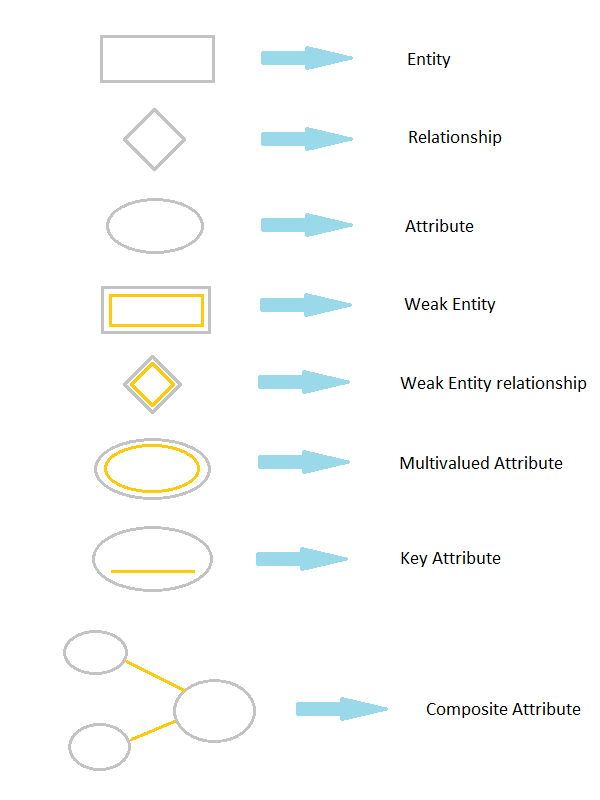
\includegraphics[width=2.7in,height=3in]{../fig/er}
\caption{Components of ER Diagram}
\end{figure}

\subsection{Entity}
An entity can be a person, place, event, or object that is relevant to a given system. For example, a school system may include students, teachers, major courses, subjects, fees and other items. Entities are represented in ER diagrams by a rectangle and named using singular nouns.

\subsection{Weak Entity}
A weak entity is an entity that depends on the existence of another entity. In more technical terms it can be defined as an entity that cannot be identified by its own attributes. It uses a foreign key combined with its attributed to form the primary key. An entity like order item is a good example for this. The order item will be meaningless without an order so it depends on the existence of the order.

\subsection{Attribute}
An attribute is a property, trait, or characteristic of an entity, relationship, or another attribute. For example, the attribute Inventory Item Name is an attribute of the entity Inventory Item. An entity can have as many attributes as necessary. Meanwhile, attributes can also have their own specific attributes. For example, the attribute “customer address” can have the attributes number, street, city, and state. These are called composite attributes. Note that some top level ER diagrams do not show attributes for the sake of simplicity. In those that do, however, attributes are represented by oval shapes.

\subsection{Multivalued Attribute}
If an attribute can have more than one value it is called a multivalued attribute. It is important to note that this is different from an attribute having its own attributes. For example, a teacher entity can have multiple subject values.

\subsection{Derived Attribute}
An attribute based on another attribute. This is found rarely in ER diagrams. For example, for a circle, the area can be derived from the radius.

\subsection{Relationship}
A relationship describes how entities interact. Relationships are represented by diamond shapes and are labelled using verbs.

\subsection{Recursive Relationship}
If the same entity participates more than once in a relationship it is known as a recursive relationship. In the below example an employee can be a supervisor and be supervised, so there is a recursive relationship.

\subsection{Cardinality Ratio}
There are three types of Cardinality Ratios:
\begin{itemize}
\item 1:1
\item 1:N
\item M:N
\end{itemize}
\begin{figure}[hbtp]
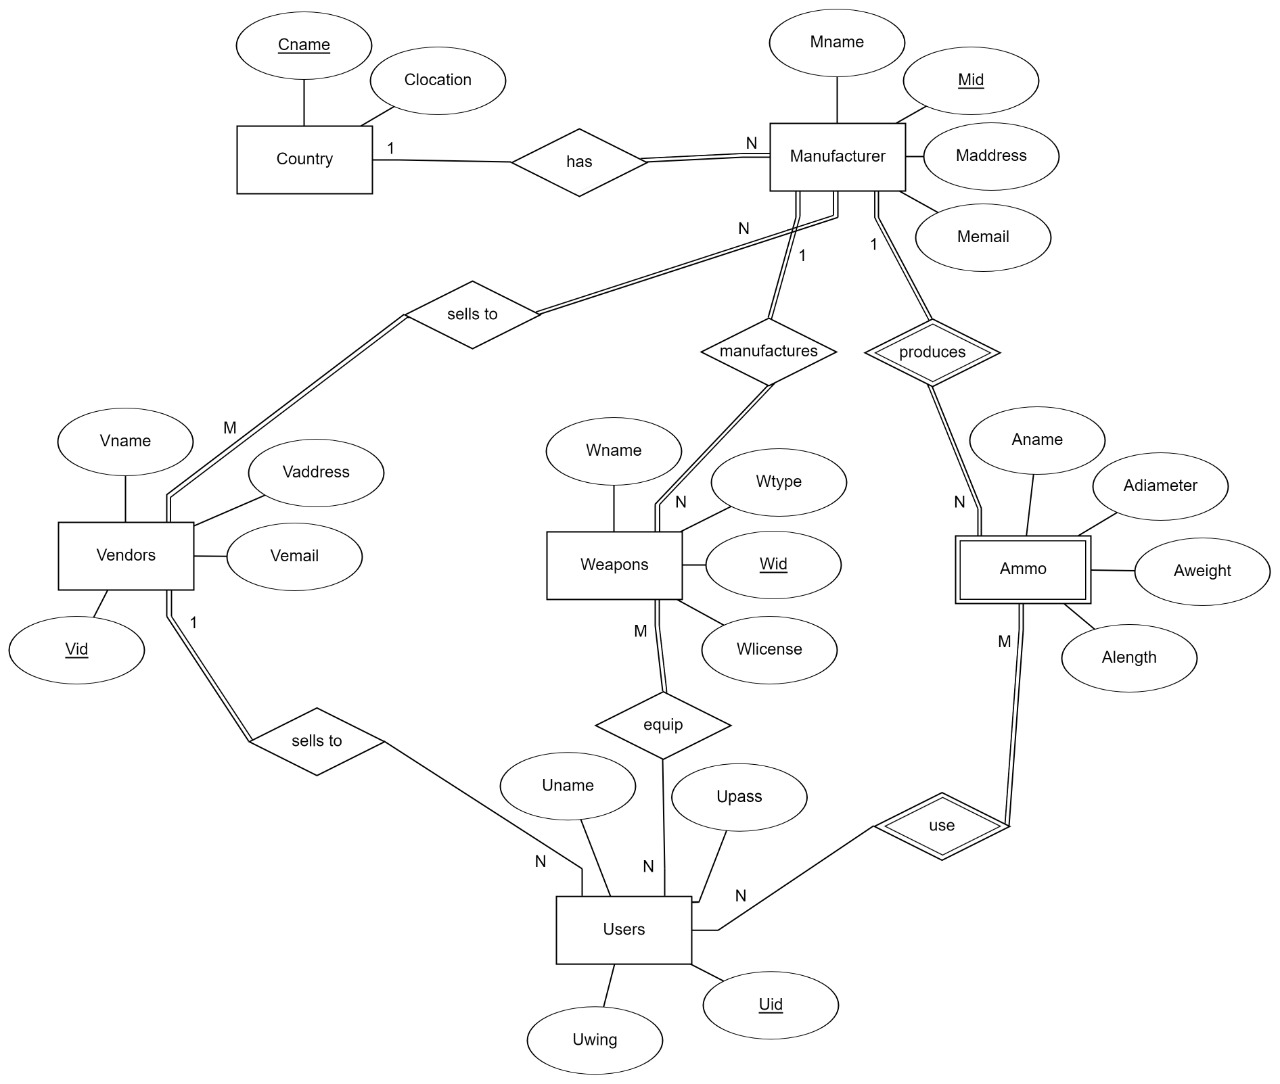
\includegraphics[width=6in,height=4.5in]{../fig/entity}
\caption{ER Diagram of Arms and Ammunition Management System}
\end{figure}

\newpage\section{Mapping From ER Diagram to Schema Diagram}
\textbf{1.Mapping of Regular Entities}:This step involves mapping all the regular entity types to tabular format by identifying their primary keys.\\
\textbf{2.Mapping of 1:1 Relation:}In this step foreign keys are assigned using foreign key approach.The primary key of the participating relation R or S is added as primary key to second entity types by looking at the participating constraints.\\
\textbf{3.Mapping of 1:N Relation:}Foreign key approach is used to add one sided primary key to the n sided entity at foreign key.\\
\textbf{4.Mapping of M:N Relation:}Here we use the cross reference approach where the relationship is converted to a new relation within attributes on primary keys of both participating relation.\\
\textbf{5.Mapping of Weak Entity:}When mapping weak entity types along with other attributes the partial key and primary key of parent entity together will form their primary key of the new relation.\\
\textbf{6.Mapping of N-ary Relation:}For mapping N array relationship we create a new relation with a relationship name in its attribute and primary keys of all participating entity types.\\
\textbf{7.Mapping of Multivalued Relation:}For multivalued attributes a separate relation has to be created along with primary key of parent relation.\\

In our database we have the following mappings:\\
\textbf{Step – 1 : Mapping of Regular Entities.}\\
From the ER diagram we identify all the strong entities E and create a relation R that includes all it’s simple attributes and primary keys.\\
The following are the strong entities from our schema diagram :\\
1.COUNTRY(\underline{Cname},Clocation)\\
2.MANUFACTURER(\underline{Mid},Mname,Maddress,Memail)\\
3.VENDORS(\underline{Vid},Vname,Vaddress,Vemail)\\
4.WEAPONS(\underline{Wid},Wname,Wtype,Wlicense)\\
5.USERS(\underline{Uid},Uname,Uwing)\\
\newpage
\begin{figure}[hbtp]
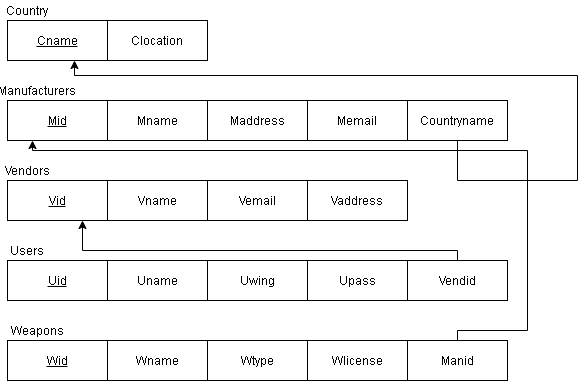
\includegraphics[width=5in,height=4.0in]{../fig/Regular}
\caption{Mapping of Regular Entities}
\end{figure}
\textbf{Step – 2 : Mapping of binary 1:1 Relation Types.}\\
In relational database design, a one-to-one (1:1) relationship exists when zero or one instance of entity A can be associated with zero or one instance of entity B, and zero or one instance of entity B can be associated with zero or one instance of entity A.\\
Unfortunately, we don't have any 1:1 relation existing within our database design.  \\

\textbf{Step – 3 : Mapping of binary 1:N Relation Types.}\\
The COUNTRY and the MANUFACTURER entities are participating in the 1:N relation 

type. Since MANUFACTURER in one the nth side of the relation we include the primary key of COUNTRY entity as the Foreign key in MANUFACTURER entity.\\
The MANUFACTURER and the WEAPONS entities are participating in the 1:N relation 

type. Since WEAPONS in one the nth side of the relation we include the primary key of MANUFACTURER entity as the Foreign key in WEAPONS entity.\\
The VENDORS and the USERS entities are participating in the 1:N relation type. Since USERS in one the nth side of the relation we include the primary key of VENDORS entity as the Foreign key in USERS entity.\\
The MANUFACTURER and the AMMOS entities are participating in the 1:N relation type. Since AMMOS in one the nth side of the relation we include the primary key of MANUFACTURER entity as the Foreign key in AMMOS entity.\\

\textbf{Step – 4 : Mapping of binary M:N Relation Types.}\\
The relationship between the VENDORS and the MANUFACTURER is M:N .So we create a new relation SELLS TO which includes the primary key of VENDORS AND MANUFACTURER entity. The combination of the two primary keys will form the primary key of the SELLS TO relation.\\

The relationship between the WEAPONS and the USERS is M:N .So we create a new relation EQUIP which includes the primary key of WEAPONS AND USERS entity. The combination of the two primary keys will form the primary key of the EQUIP relation.\\

\begin{figure}[hbtp]
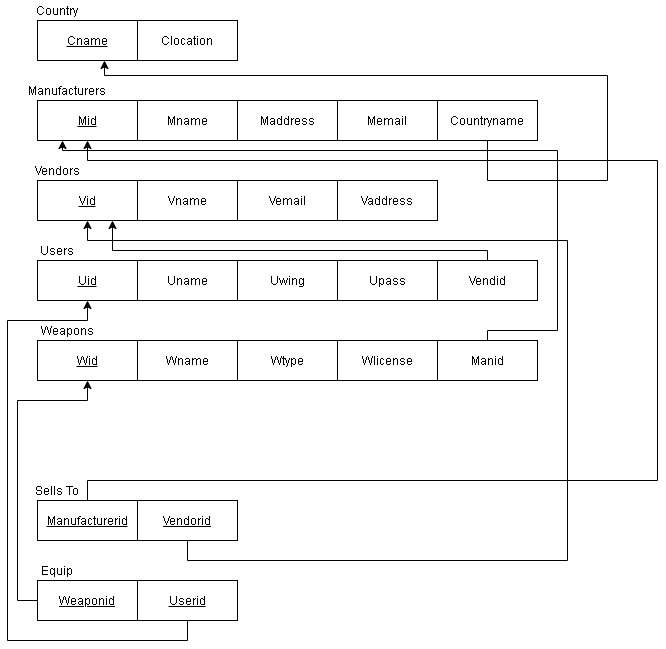
\includegraphics[width=6in,height=4.5in]{../fig/M-N}
\caption{Mapping of binary M:N Relation Types}
\end{figure}
\newpage
\textbf{Step – 5 : Mapping of Weak Entity.}\\
From the ER diagram we identify all the weak entities E and create a relation R that includes all it’s simple attributes and partial keys.\\
The following are the weak entities from our schema diagram :\\
1.AMMOS(\underline{Aname},Adiameter,Aweight,Alength)
\begin{figure}[hbtp]
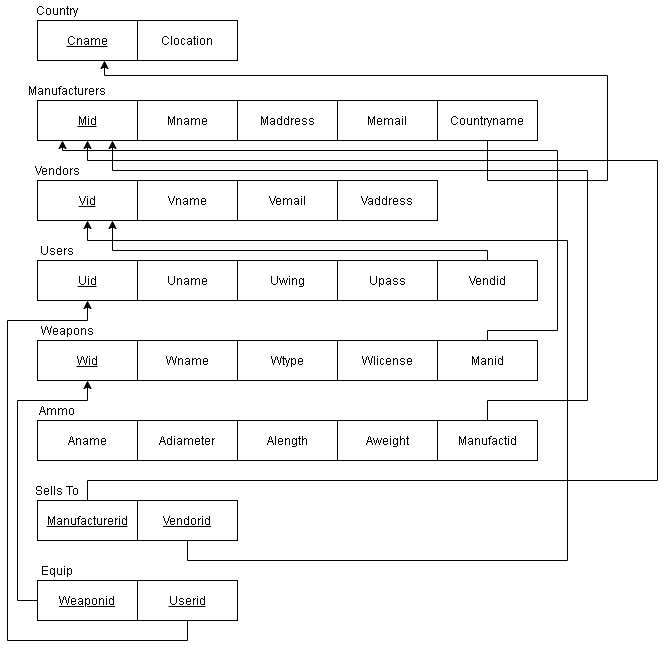
\includegraphics[width=6in,height=5.0in]{../fig/RS}
\caption{Mapping of Weak Entity}
\end{figure}
\section{Schema Diagram}
\par
A Schema is a pictorial representation of the relationship between the database tables in the database that is created. The database schema of a database system is its structure described in a formal language sup ported by the database management system (DBMS). The term "schema" refers to the organization of data as a blueprint of how the database is constructed (divided into database tables in the case of relational databases). \\
The formal definition of a database schema is a set of formulas (sentences) called integrity constraints imposed on a database. These integrity constraints ensure compatibility between parts of the schema. All constraints are expressible in the same language. A database can be considered a structure in realization of the database language.The states of a created conceptual schema are transformed into an explicit mapping, the database schema. This describes how real-world entities are modelled in the database.
\\\\

\begin{figure}[hbtp]
\centering
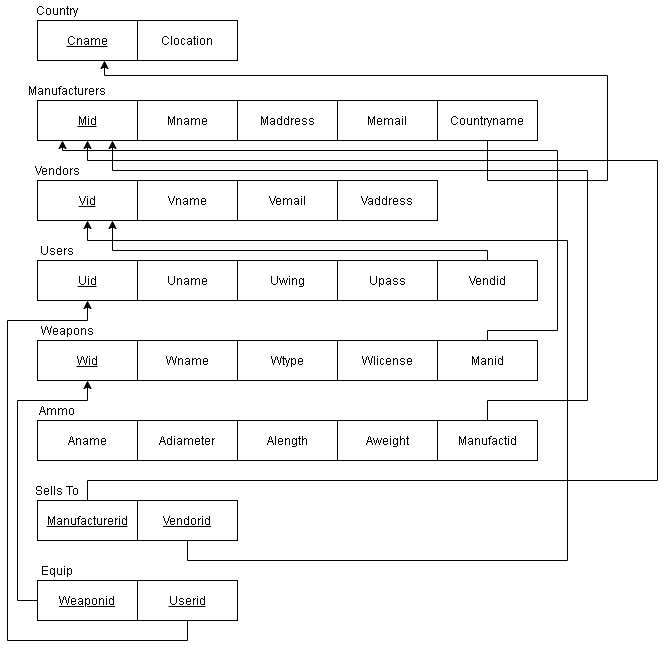
\includegraphics[width=6in,height=5.0in]{../fig/RS}
\caption{Schema Diagram of Arms and Ammunition Management System}
\end{figure}


\chapter{Implementation}
\section{Table Structure}
\textbf{AMMOS}\\
CREATE TABLE `ammos` (\\
  `Aname` varchar(50) NOT NULL,\\
  `Adiameter` varchar(20) NOT NULL,\\
  `Alength` varchar(20) NOT NULL,\\
  `Aweight` varchar(20) NOT NULL,\\
  `Manufactid` int(10) NOT NULL\\
) ENGINE=InnoDB DEFAULT CHARSET=latin1;\\
ALTER TABLE `ammos`\\
  ADD CONSTRAINT `Manufactid` FOREIGN KEY\\ (`Manufactid`) REFERENCES `manufacturers` (`Mid`) ON DELETE CASCADE ON UPDATE CASCADE;
\begin{figure}[hbtp]
\centering
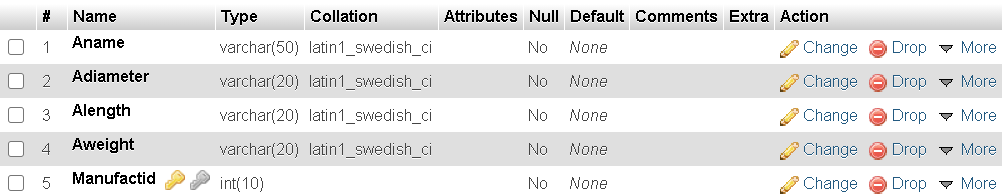
\includegraphics[width=6.0in,height=2in]{../fig/Ammos}\\
\end{figure}\\
\newpage
\textbf{COUNTRY}\\
CREATE TABLE `country` (\\
  `Cname` varchar(50) NOT NULL,\\
  `Clocation` varchar(50) NOT NULL\\
) ENGINE=InnoDB DEFAULT CHARSET=latin1;\\
ALTER TABLE `country`\\
ADD PRIMARY KEY (`Cname`);
\begin{figure}[hbtp]
\centering
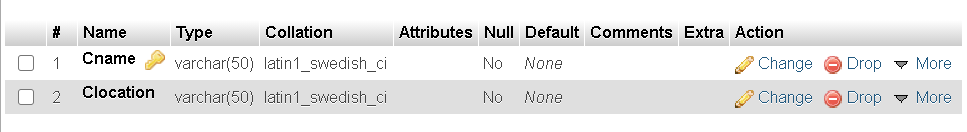
\includegraphics[width=6.0in,height=1.25in]{../fig/Country}\\
\end{figure}
\begin{flushleft}
\textbf{EQUIP}\\
CREATE TABLE `equip` (\\
  `Weaponid` int(10) NOT NULL,\\
  `Userid` int(10) NOT NULL\\
) ENGINE=InnoDB DEFAULT CHARSET=latin1;\\
ALTER TABLE `equip`\\
  ADD CONSTRAINT `Userid` FOREIGN KEY (`Userid`) REFERENCES `users` (`Uid`) ON DELETE CASCADE ON UPDATE CASCADE,\\
  ADD CONSTRAINT `Weaponid` FOREIGN KEY (`Weaponid`) REFERENCES `weapons` (`Wid`) ON DELETE CASCADE ON UPDATE CASCADE;
\end{flushleft}
\begin{figure}[hbtp]
\centering
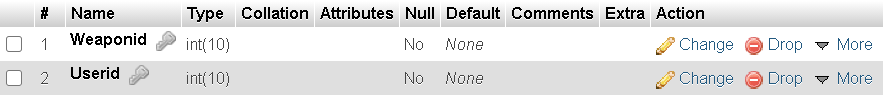
\includegraphics[width=6.0in,height=1.0in]{../fig/Equip}\\
\end{figure}
\begin{flushleft}
\newpage
\textbf{MANUFACTURER}\\
CREATE TABLE `manufacturers` (\\
  `Mid` int(10) NOT NULL,\\
  `Mname` varchar(50) NOT NULL,\\
  `Maddress` varchar(50) NOT NULL,\\
  `Memail` varchar(50) NOT NULL,\\
  `Countryname` varchar(50) NOT NULL\\
) ENGINE=InnoDB DEFAULT CHARSET=latin1;\\
ALTER TABLE `manufacturers`\\
  ADD PRIMARY KEY (`Mid`),\\
  ADD KEY `Countryname` (`Countryname`);\\
ALTER TABLE `manufacturers`\\
  ADD CONSTRAINT `Countryname` FOREIGN KEY (`Countryname`) REFERENCES `country` (`Cname`) ON DELETE CASCADE ON UPDATE CASCADE;
\end{flushleft}
\begin{figure}[hbtp]
\centering
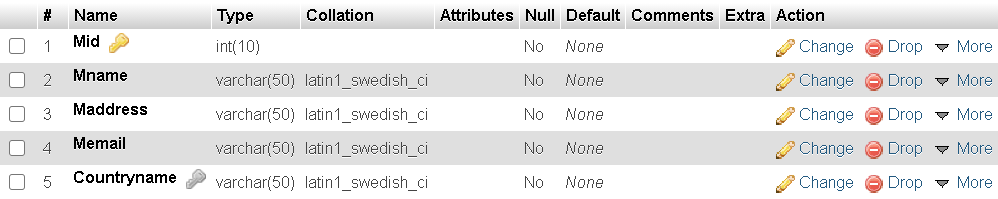
\includegraphics[width=6.0in,height=2in]{../fig/Manufacturer}\\
\end{figure}
\begin{flushleft}
\newpage
\textbf{SELLS TO}\\
CREATE TABLE `sellsto` (\\
  `Manufactureid` int(10) NOT NULL,\\
  `Vendorid` int(10) NOT NULL\\
) ENGINE=InnoDB DEFAULT CHARSET=latin1;\\
ALTER TABLE `sellsto`\\
  ADD KEY `Manufactureid` (`Manufactureid`),\\
  ADD KEY `Vendorid` (`Vendorid`);\\
  ALTER TABLE `sellsto`\\
  ADD CONSTRAINT `Manufactureid` FOREIGN KEY (`Manufactureid`) REFERENCES `manufacturers` (`Mid`) ON DELETE CASCADE ON UPDATE CASCADE,\\
  ADD CONSTRAINT `Vendorid` FOREIGN KEY (`Vendorid`) REFERENCES `vendors` (`Vid`) ON DELETE CASCADE ON UPDATE CASCADE;
\end{flushleft}
\begin{figure}[hbtp]
\centering
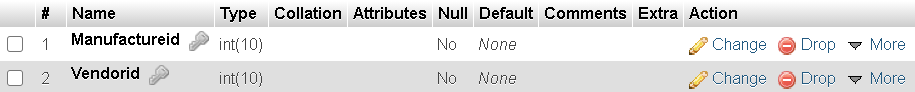
\includegraphics[width=6.0in,height=1.0in]{../fig/Sellsto}\\
\end{figure}
\begin{flushleft}
\newpage
\textbf{USERS}\\
CREATE TABLE `users` (\\
  `Uid` int(10) NOT NULL,\\
  `Uname` varchar(100) NOT NULL,\\
  `Uwing` varchar(50) NOT NULL,\\
  `Upass` varchar(100) NOT NULL,\\
  `Vendid` int(10) NOT NULL\\
) ENGINE=InnoDB DEFAULT CHARSET=latin1;\\
ALTER TABLE `users`\\
  ADD PRIMARY KEY (`Uid`),\\
  ADD KEY `Vendid` (`Vendid`);\\
 ALTER TABLE `users`\\
  ADD CONSTRAINT `Vendid` FOREIGN KEY (`Vendid`) REFERENCES `vendors` (`Vid`) ON DELETE CASCADE ON UPDATE CASCADE;
\end{flushleft}
\begin{figure}[hbtp]
\centering
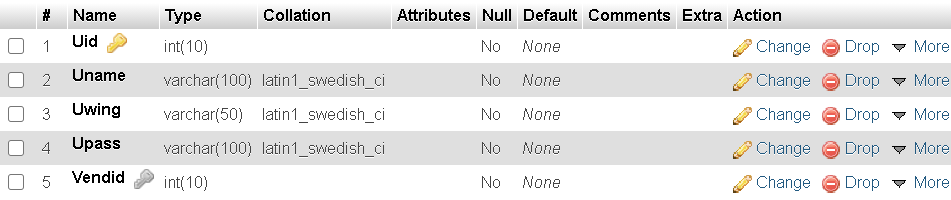
\includegraphics[width=6.0in,height=2in]{../fig/User}\\
\end{figure}
\newpage
\textbf{VENDORS}\\
CREATE TABLE `vendors` (\\
  `Vid` int(10) NOT NULL,\\
  `Vname` varchar(20) NOT NULL,\\
  `Vemail` varchar(50) NOT NULL,\\
  `Vaddress` varchar(50) NOT NULL\\
) ENGINE=InnoDB DEFAULT CHARSET=latin1;\\
ALTER TABLE `vendors`\\
  ADD PRIMARY KEY (`Vid`);
\begin{figure}[hbtp]
\centering
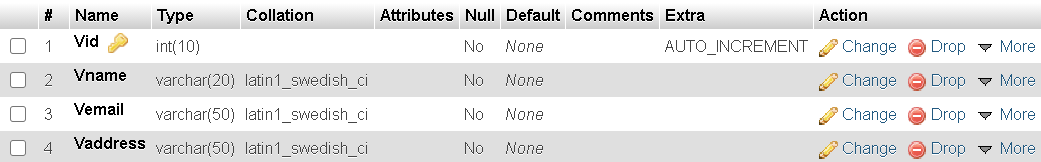
\includegraphics[width=6.0in,height=1.75in]{../fig/Vendor}\\
\end{figure}\\
\newpage
\textbf{WEAPONS}\\
CREATE TABLE `weapons` (\\
  `Wid` int(10) NOT NULL,\\
  `Wname` varchar(40) NOT NULL,\\
  `Wtype` varchar(40) NOT NULL,\\
  `Wlicense` varchar(20) NOT NULL,\\
  `Manid` int(10) NOT NULL\\
) ENGINE=InnoDB DEFAULT CHARSET=latin1;\\
ALTER TABLE `weapons`\\
  ADD PRIMARY KEY (`Wid`),\\
  ADD KEY `Manid` (`Manid`);\\
  ALTER TABLE `weapons`\\
  ADD CONSTRAINT `Manid` FOREIGN KEY (`Manid`) REFERENCES `manufacturers` (`Mid`) ON DELETE CASCADE ON UPDATE CASCADE;
\begin{figure}[hbtp]
\centering
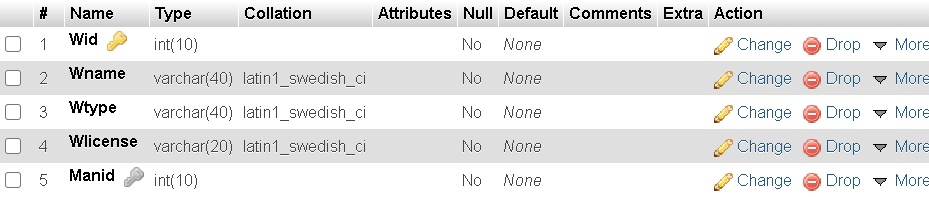
\includegraphics[width=6.0in,height=2in]{../fig/Weapons}\\
\end{figure}\\
\newpage
\section{Codes Used For Modules:}
\begin{flushleft}
\textbf{Insert}\\
\end{flushleft}
\begin{figure}[hbtp]
\centering
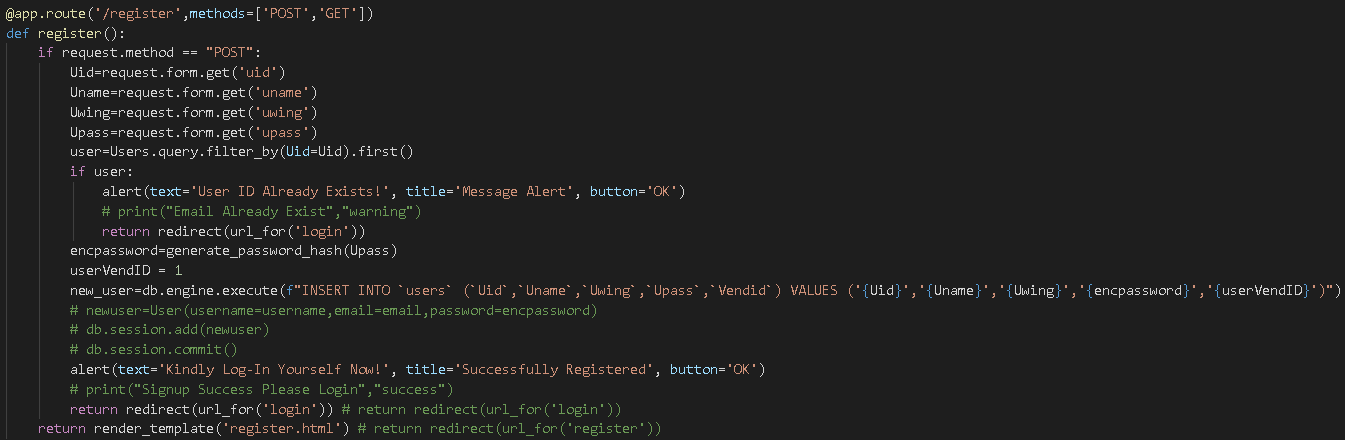
\includegraphics[width=6in,height=2in]{../fig/Inser}\\
\end{figure}
\begin{flushleft}
\textbf{Delete}\\
\end{flushleft}
\begin{figure}[hbtp]
\centering
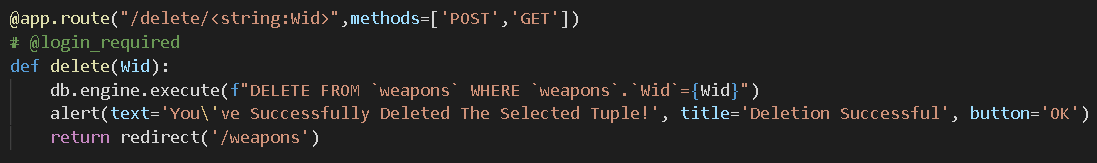
\includegraphics[width=6in,height=2in]{../fig/Delete}\\
\end{figure}
\newpage
\begin{flushleft}
\textbf{Update}\\
\end{flushleft}
\begin{figure}[hbtp]
\centering
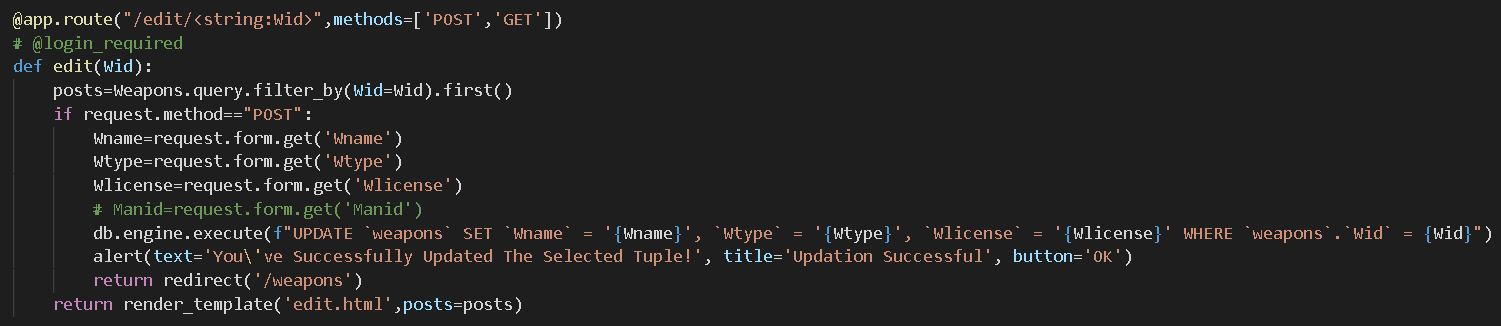
\includegraphics[width=6in,height=2in]{../fig/Update}\\
\end{figure}
\begin{flushleft}
\textbf{Search}\\
\end{flushleft}
\begin{figure}[hbtp]
\centering
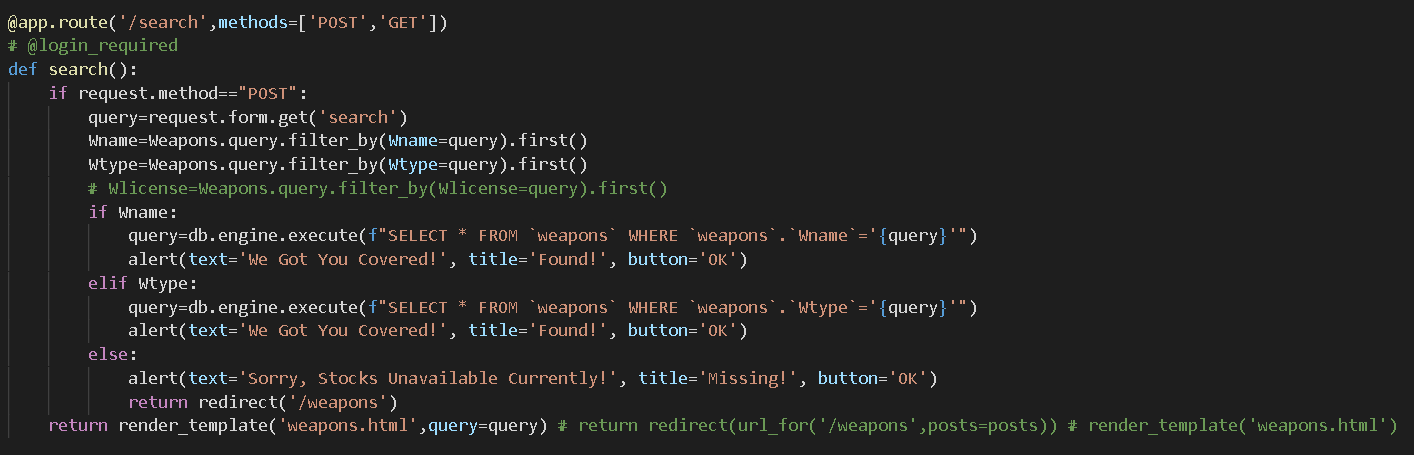
\includegraphics[width=6in,height=2in]{../fig/Search}\\
\end{figure}
\begin{flushleft}
\textbf{Display}\\
\end{flushleft}
\begin{figure}[hbtp]
\centering
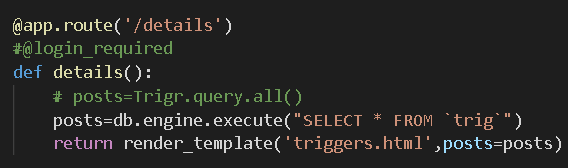
\includegraphics[width=6in,height=2in]{../fig/All}\\
\end{figure}
\newpage
\begin{flushleft}
\textbf{Trigger}\\
CREATE TRIGGER `weaponDeletion` BEFORE DELETE ON `weapons` \\FOR EACH ROW INSERT INTO trig VALUES(null,OLD.Wid,OLD.Wname,OLD.Wtype,OLD.Wlicense,'Weapon Deleted!',NOW())\\
CREATE TRIGGER `weaponInsertion` AFTER INSERT ON `weapons` \\FOR EACH ROW INSERT INTO trig
VALUES(null,NEW.Wid,NEW.Wname,NEW.Wtype,NEW.Wlicense,'Weapon Inserted!',NOW())\\
CREATE TRIGGER `weaponUpdation` AFTER UPDATE ON `weapons` \\FOR EACH ROW INSERT INTO trig 
VALUES(null,NEW.Wid,NEW.Wname,NEW.Wtype,NEW.Wlicense,'Weapon Info Updated!',NOW())\\
\end{flushleft}

\chapter{Results and Discussion}
\textbf{Login Page:}\\
\begin{figure}[hbtp]
\centering
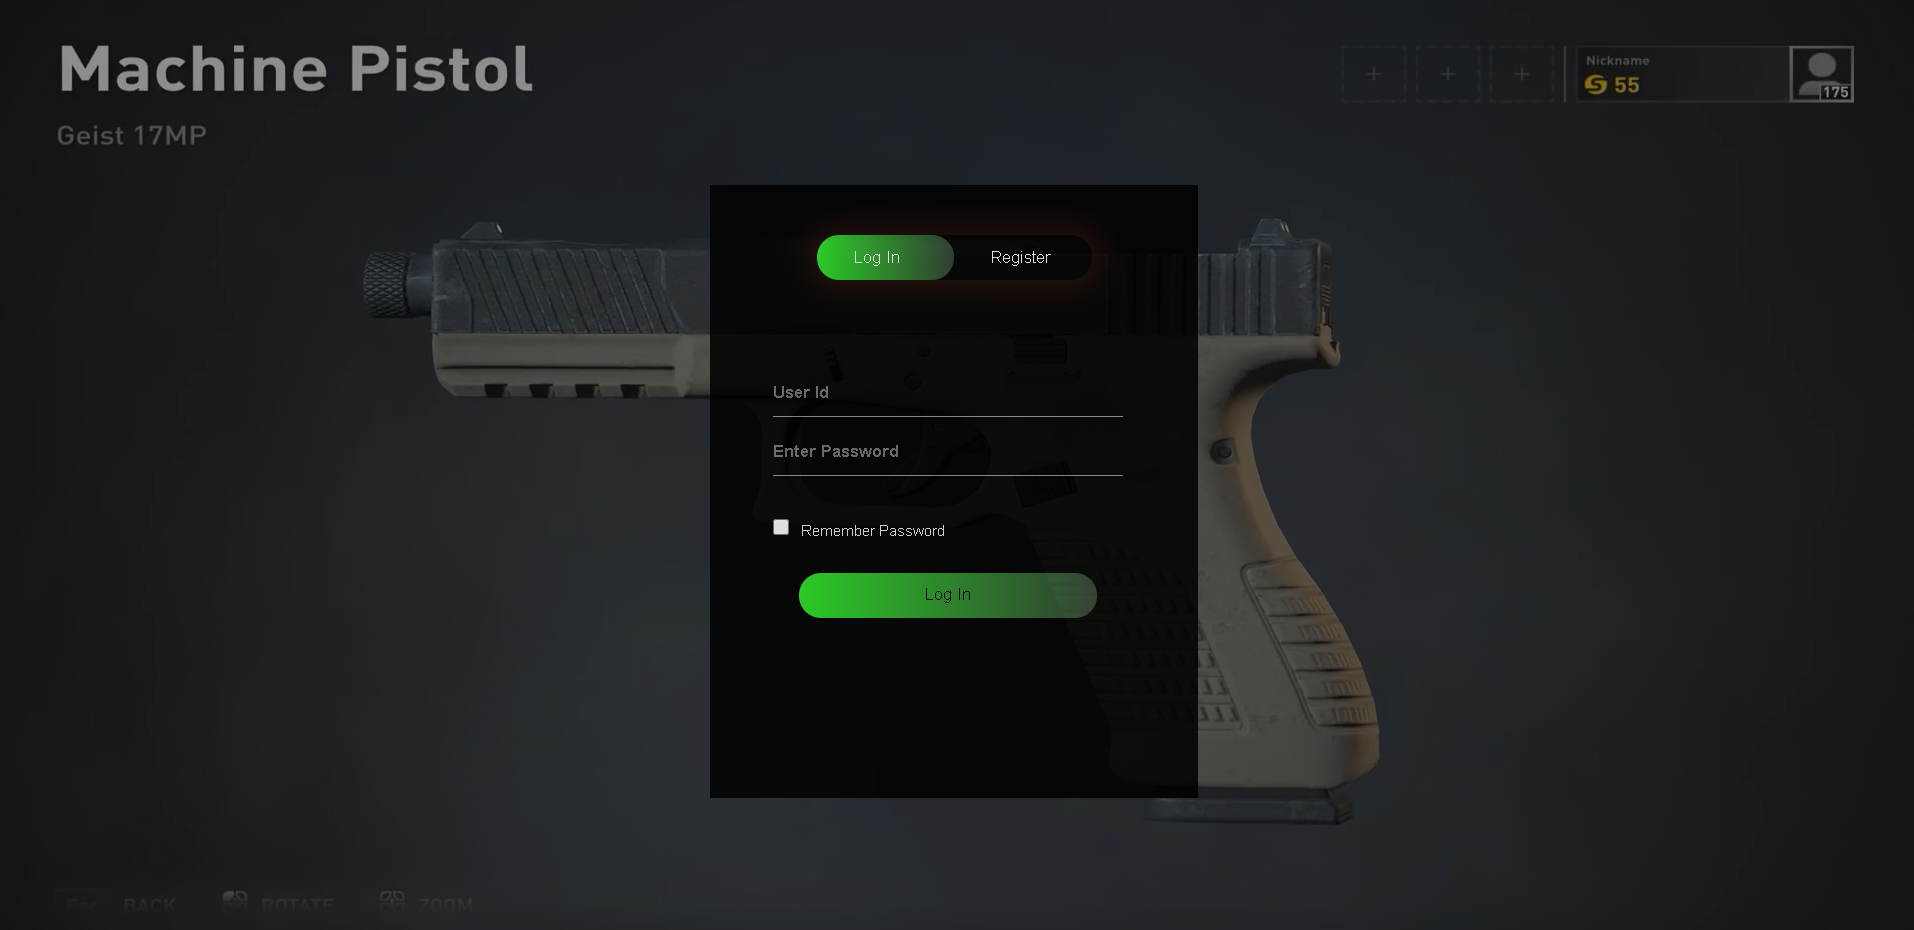
\includegraphics[width=4.5in,height=2in]{../fig/Log}
\caption{Login Page}
\end{figure}\\
\noindent
This is our login page. Here the User can enter his Id and login.\\
%-----------------------
\textbf{Registration Page:}\\
\begin{figure}[hbtp]
\centering
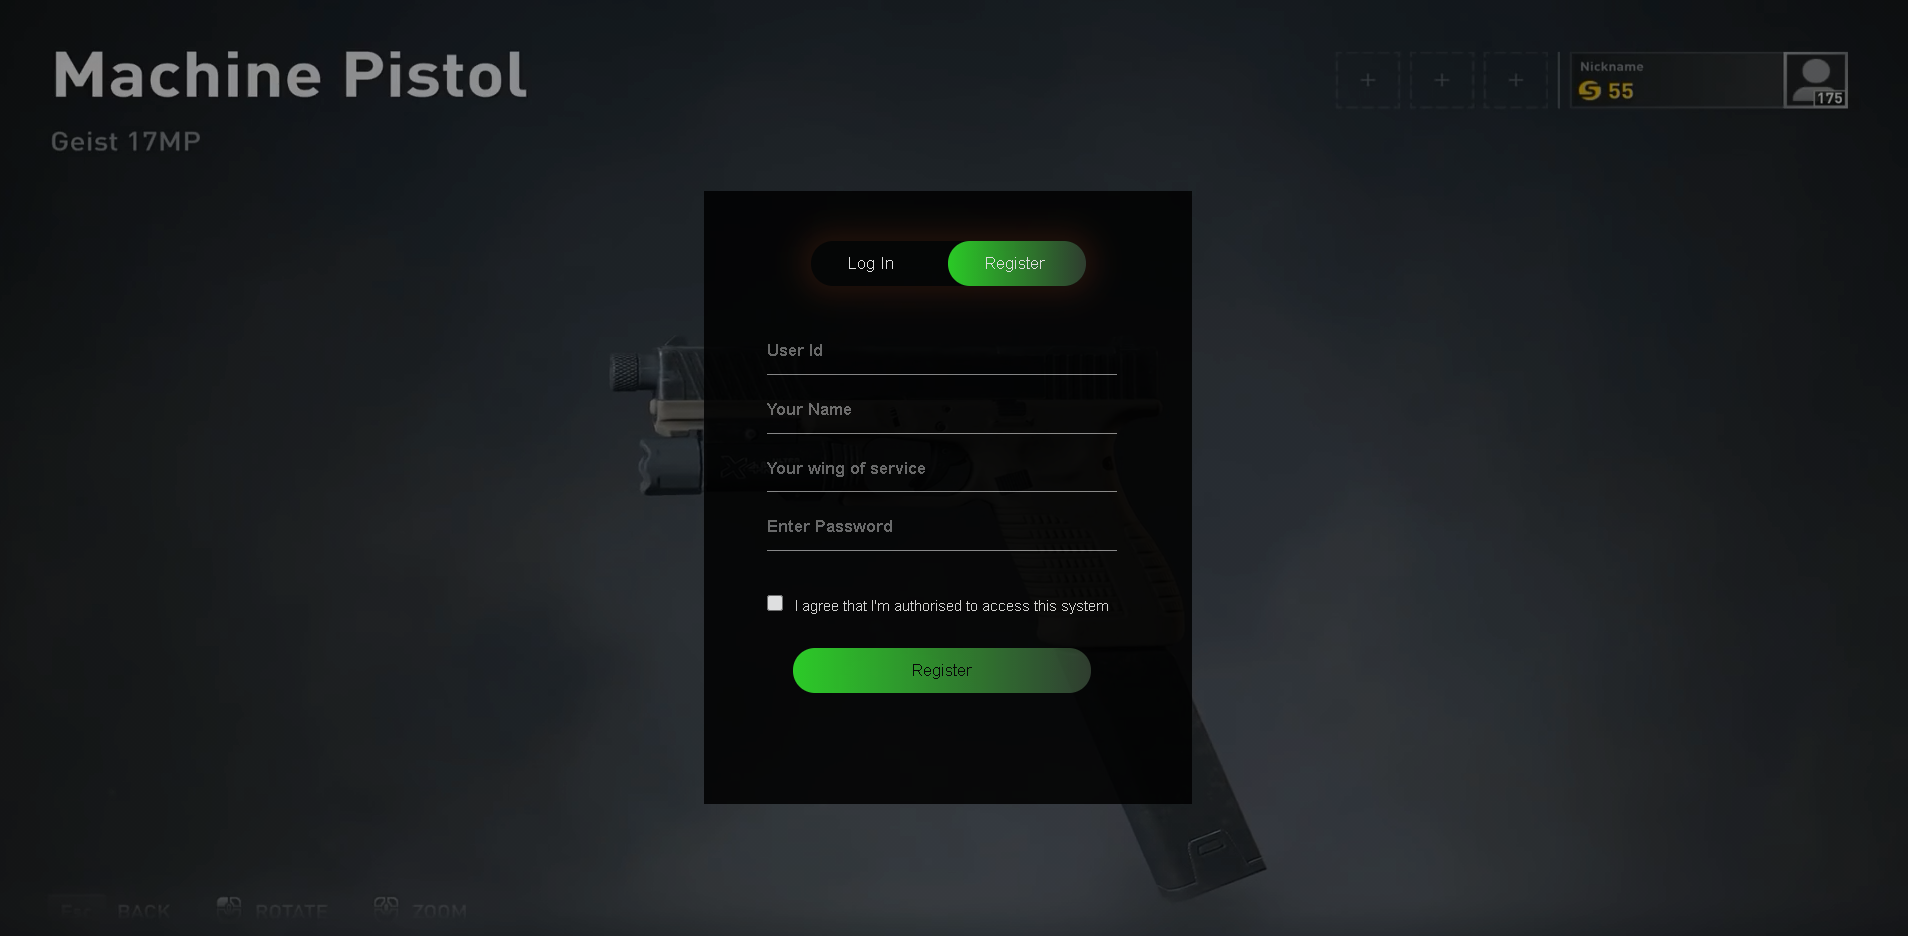
\includegraphics[width=4.5in,height=2in]{../fig/Reg}
\caption{Registration Page}
\end{figure}\\
\noindent
This page allows a new User to have access to the database.
\newpage
%-----------------------
\textbf{Deleting Weapons:}\\
\begin{figure}[hbtp]
\centering
\includegraphics[width=6in,height=2in]{../fig/deletee}\\
\caption{Delete Weapons}
\end{figure}\\
\noindent
Here User can delete the weapons of certain manufacturers by selecting that particular row.\\

%-----------------------
\textbf{Update Weapon Details:}\\
\begin{figure}[hbtp]
\centering
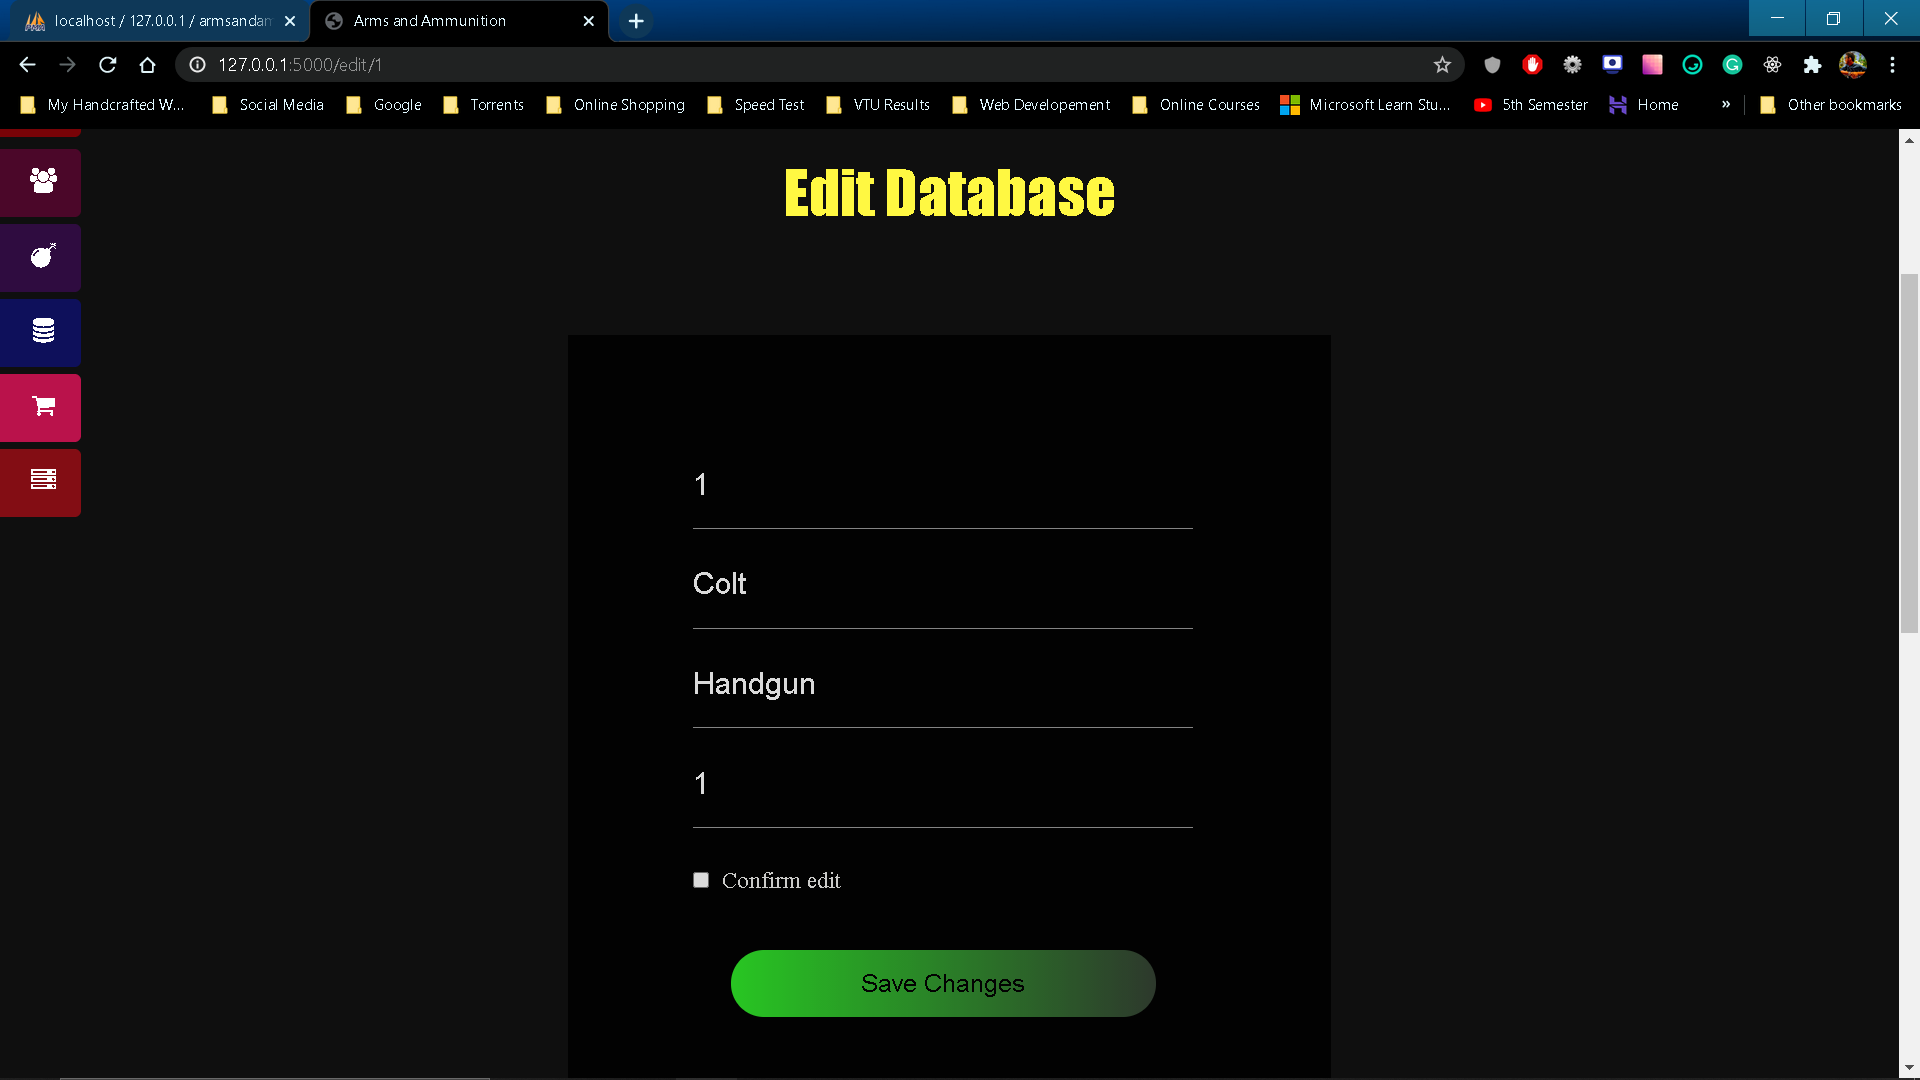
\includegraphics[width=6in,height=2in]{../fig/updatee}\\
\caption{Update Weapon Details}
\end{figure}\\
\noindent
Here User can update the details of certain weapons.\\

\newpage
%-----------------------
\textbf{Search Weapon Details:}\\
\begin{figure}[hbtp]
\centering
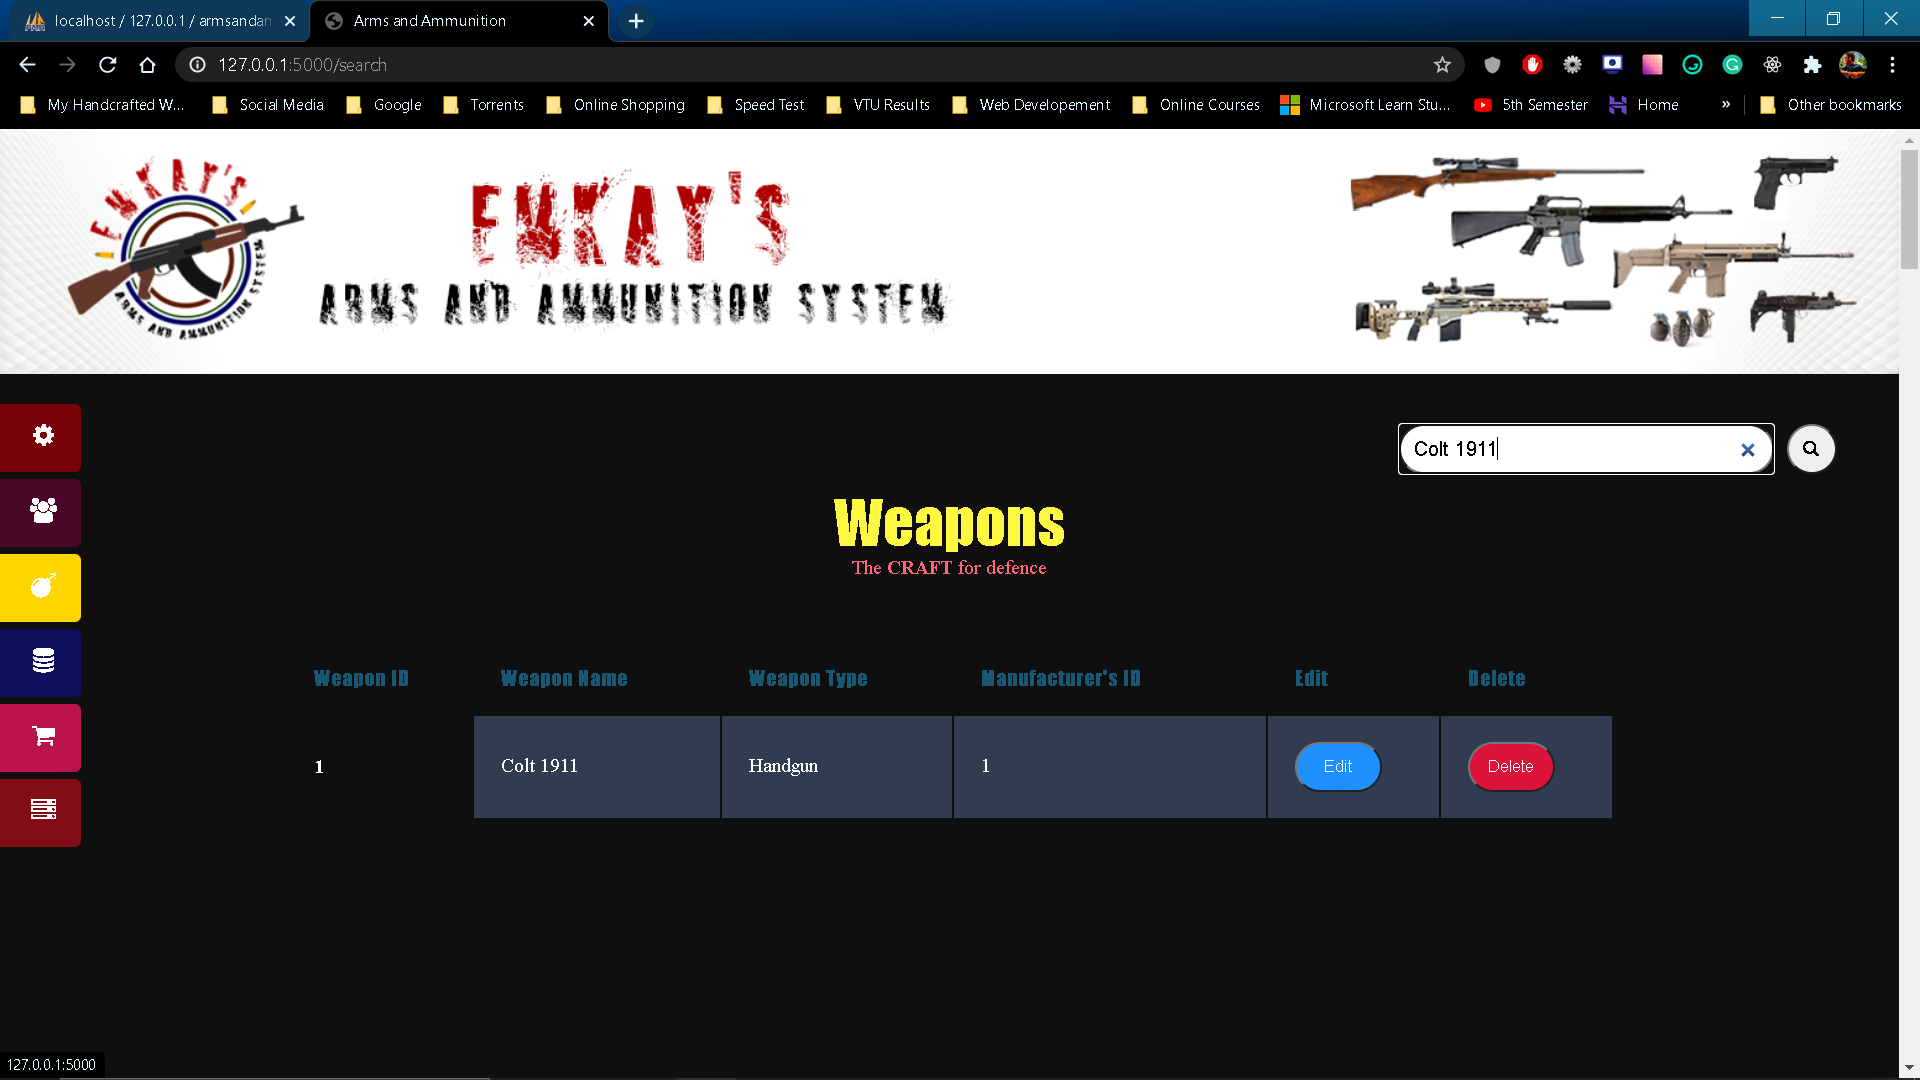
\includegraphics[width=6in,height=2in]{../fig/searchh}\\
\caption{Search Weapon Details}
\end{figure}\\
\noindent
Here User can search for the details of certain weapons using type or name of the weapon.\\

%----------------------
\textbf{Trigger:}\\
\begin{figure}[hbtp]
\centering
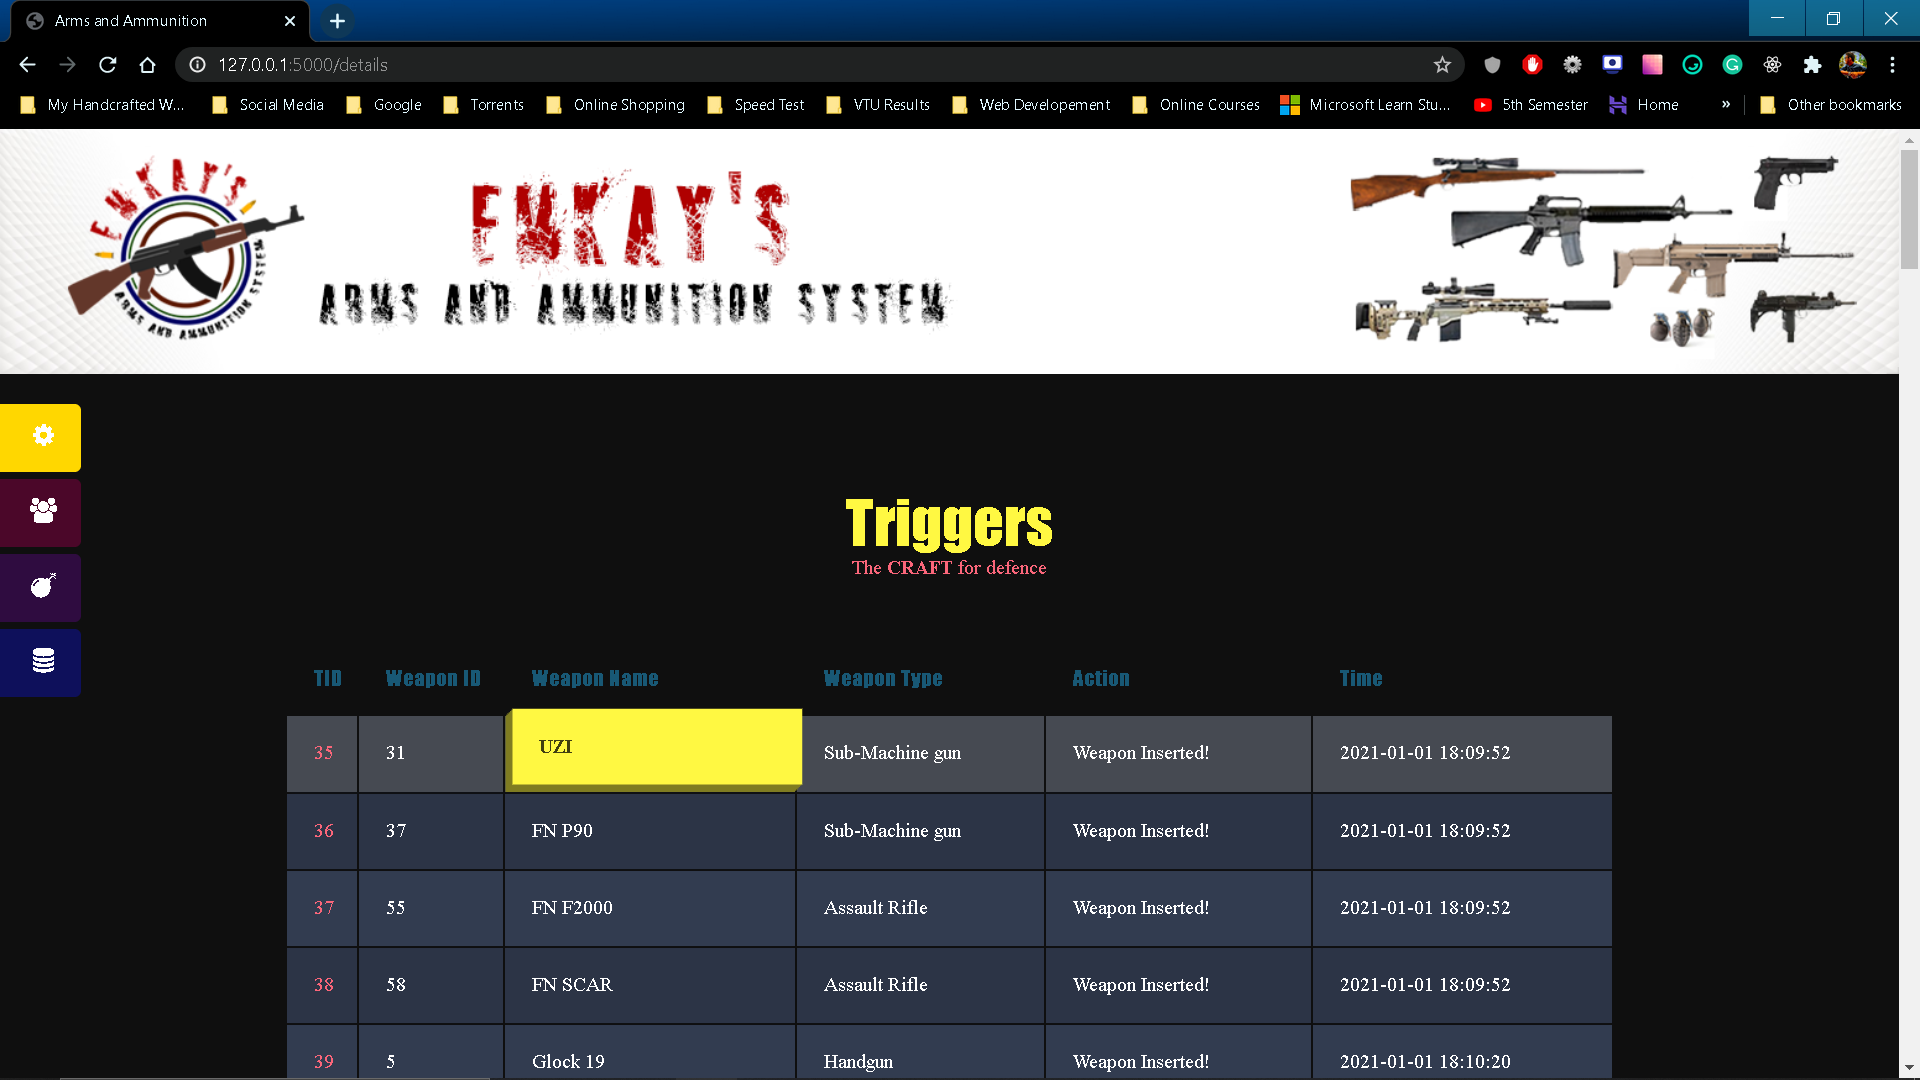
\includegraphics[width=6in,height=2in]{../fig/Trigger}\\
\caption{Trigger for Modification of Weapons}
\end{figure}\\
\noindent
Trigger will be violated if anyone modifies certain attributes of weapons.\\
\newpage

%---------------------
\textbf{Mail:}\\
\begin{figure}[hbtp]
\centering
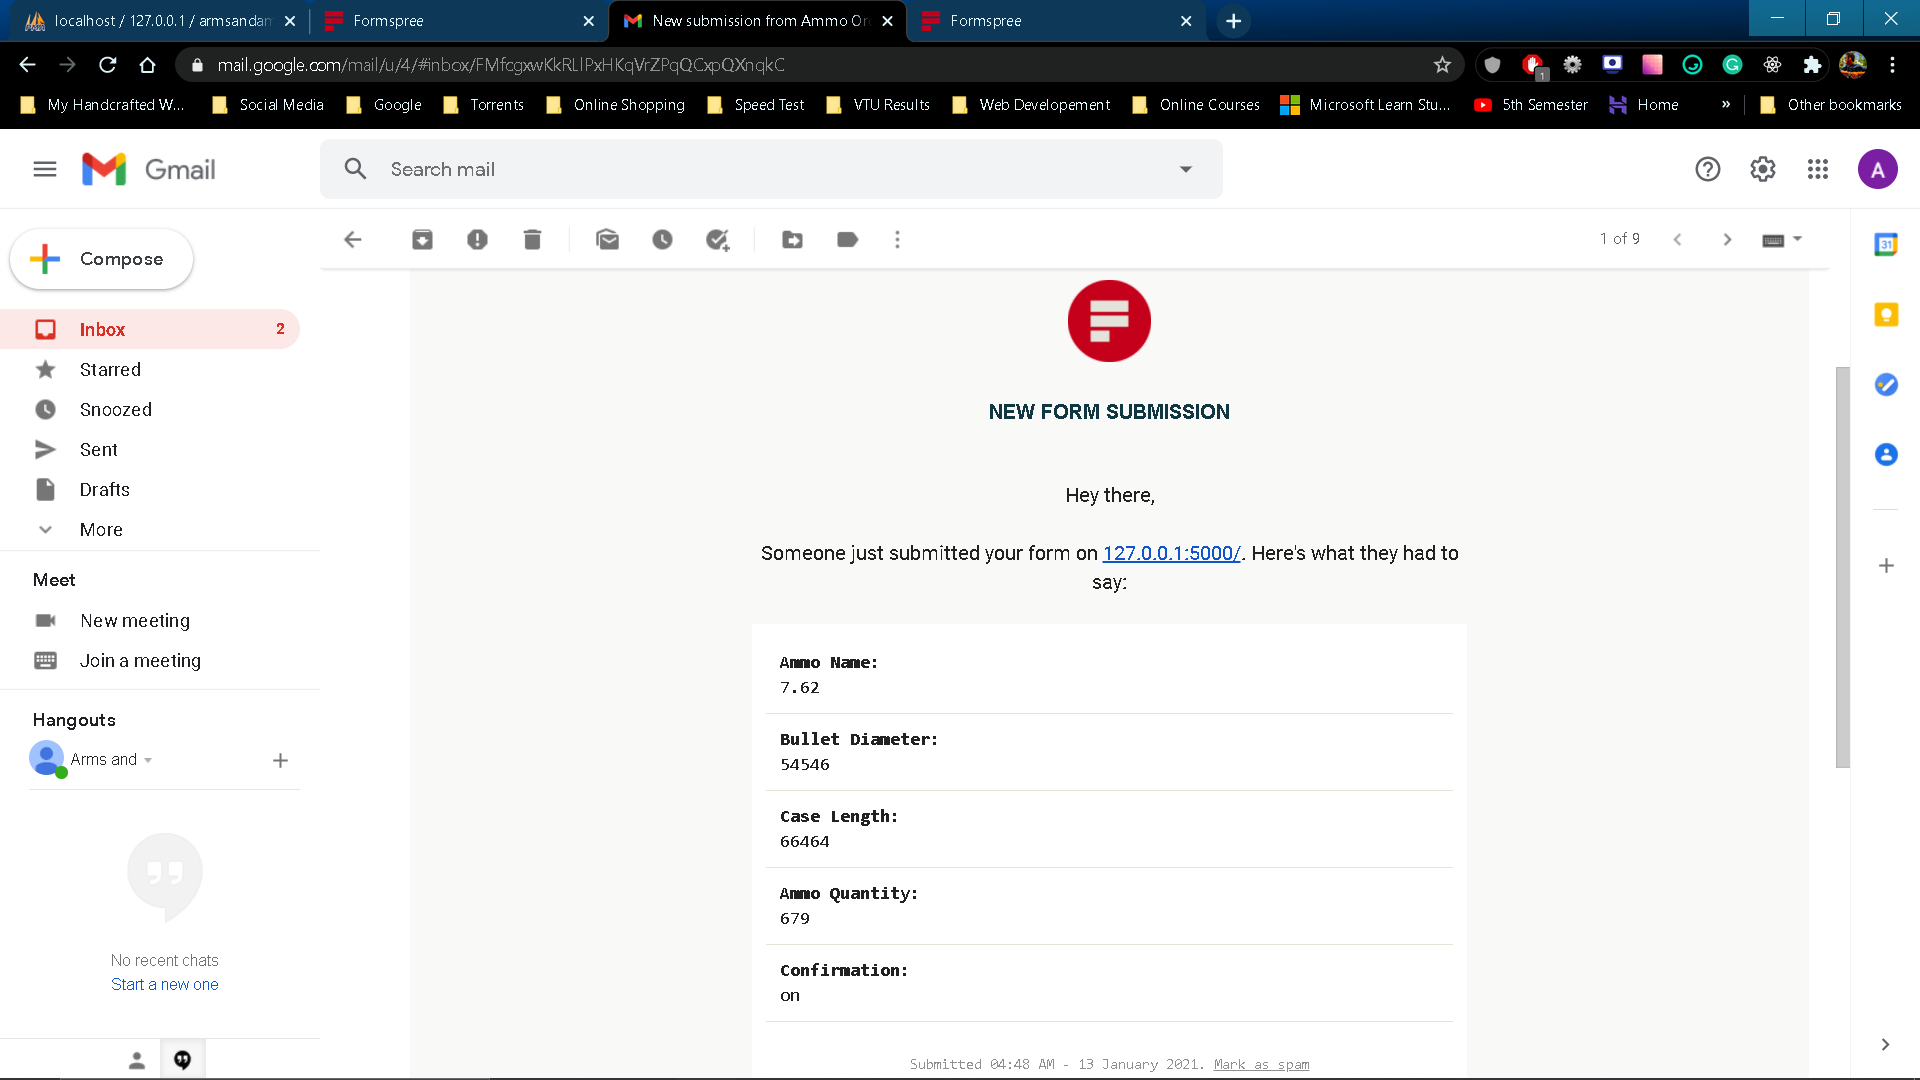
\includegraphics[width=6in,height=2in]{../fig/mail}
\caption{Mail Generated}
\end{figure}\\
\noindent
Generating the mail.

%---------------------
\chapter{Conclusion and Future work}
\noindent
The small and medium-sized Arms and Ammunition system is using Python-Flask \\SQLAlchemy Toolkit to develop and realize procurement and inventory management has always been an essential part of the weapons. Arms and Ammunition Management System realizes the function of procurement management, inventory management, sales management, user management and membership management that Army needed. With the continuous improvement of science and technology, the computer's powerful function has been known and used. Compared with the old manual work, the system not only reduces the workload, but also greatly reduced the occurrence of human error. 
\noindent
This project can be further improved by differentiating user and admin interfaces so that a recruit might not alter the database and only an experienced officer can administrate the system.
Keeping track of when the user or the manufacturer was registered or deleted, giving a warning when
the weapon and ammos quantity goes low. Keeping a track of the sales that have happened on a particular day.
\newpage
\pagestyle{plain}
\renewcommand{\bibname}{References}
\bibliography{references}
\addcontentsline{toc}{chapter}{References}
\begin{thebibliography}{35}
\bibitem{ds}Database systems Models, Languages, Design and Application Programming, Ramez Elmasri and Shamkant B. Navathe, 6th Edition, Pearson.

\bibitem{dm}Database management systems, Ramakrishnan, and Gehrke, 3rd Edition, 2014, McGraw Hill.

\bibitem{korth}Silberschatz Korth and Sudharshan: Database System Concepts, 6th Edition, Mc-Graw Hill, 2013.

\bibitem{mor}Coronel, Morris, and Rob, Database Principles Fundamentals of Design, Implementation and  
Management, Cengage Learning 2012.

\end{thebibliography}

\end{document}